% Name: Array
% Description: An array of eight integers in consecutive cells, with each cell's index below and a pointer to the element being read.
% Tags: array, index, memory, data structures

\usetikzlibrary{arrows.meta, positioning}

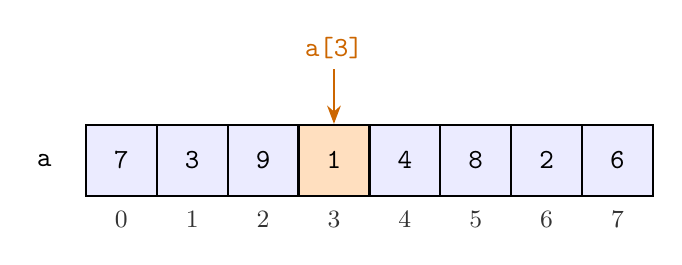
\begin{tikzpicture}[>={Stealth}, cell/.style={draw, thick, minimum size=9mm, font=\ttfamily}]
  \foreach \v [count=\i from 0] in {7, 3, 9, 1, 4, 8, 2, 6} {
    \node[cell, fill=blue!8] (a\i) at (\i*0.9,0) {\v};
    \node[font=\small, gray!40!black] at (\i*0.9,-0.75) {\i};
  }
  \node[cell, fill=orange!25] at (a3) {1};
  \node[left=3mm of a0, font=\ttfamily] {a};
  \draw[<-, thick, orange!80!black] (a3.north) -- ++(0,0.7) node[above, font=\ttfamily] {a[3]};
\end{tikzpicture}
